\documentclass[11pt]{article}

% ---------- fonts & layout ----------
\usepackage[T1]{fontenc}
\usepackage[utf8]{inputenc}
\usepackage[margin=1in]{geometry}
\usepackage{amsmath,amssymb,amsthm}
\let\Bbbk\relax                    % avoid newtxmath/amssymb \Bbbk clash
\usepackage{newtxtext,newtxmath}   % Times-like, professional (after amssymb)
\usepackage{microtype}
\usepackage{booktabs}
\usepackage{graphicx}
\usepackage{xcolor}
\usepackage{enumitem}
\usepackage[numbers,square,comma]{natbib}
\usepackage{tikz}
\usetikzlibrary{arrows.meta,positioning,fit,backgrounds,calc}
\usepackage[hidelinks]{hyperref}
\usepackage{caption}
\captionsetup{font=small,labelfont=bf}
\graphicspath{{figures/}}

\newcommand{\Hk}{\widehat{H}\!\left(S \mid \tau_{:k}\right)}
\newcommand{\strat}{S}
\newcommand{\prefix}{\tau_{:k}}

\title{\textbf{When Do LLM Code Agents Commit to a Strategy?\\
A Counterfactual Measure of Strategic Commitment\\ via Conditional Outcome Entropy}}
\author{Ramtin Sirjani\\[2pt]
\small Western University}
\date{\small Working draft --- Introduction \& Methods (pre-experiment); \today}

\begin{document}
\maketitle

\begin{abstract}
\noindent
Test-time diversity helps multi-step language-model agents explore alternative
solutions, but in a trajectory of dozens of steps it is unclear \emph{where}
injecting diversity is worth the compute. We hypothesize that an agent
progressively \emph{commits}: as its trajectory unfolds the distribution over final
solutions narrows (mode collapse increasing with accumulated context). We introduce
a causal, non-circular measure of strategic commitment: the \emph{conditional
semantic entropy of the final strategy given the trajectory prefix},
$H(S \mid \tau_{:k})$, estimated by fixing the first $k$ steps, resampling $M$
independent continuations to completion, and measuring the semantic entropy of their
final outcomes. This is the agent-trajectory, entropy-generalized analogue of the
\emph{committor} from transition-path theory---the probability a path reaches one
basin before another---but for a \emph{learned} generator, which forces a
distinction the physical committor never had: the prefix $f^\ast$ where the model's
\emph{own} resampling collapses (it stops exploring) can precede the prefix
$f^\dagger$ where the outcome is causally \emph{locked} (no intervention can
change it). The object we actually track is the per-step \emph{leverage}---the
mutual information between a step and the final outcome---whose elementary bound
$\ell_k\le\min(\text{step branchiness},\,\text{residual outcome entropy})$ explains
why diversity pays only at a few, possibly scattered, steps rather than a contiguous
window; $f^\ast\!\le\!f^\dagger$ summarize it, ordered rigorously through reachable
\emph{support} (not an entropy inequality), and we align trajectories by the fraction
of outcome entropy resolved rather than by wall-clock step. Because a single model conflates an early-committing
\emph{problem} with a mode-collapsed \emph{model}, we estimate the curve across a
panel of models, yielding an \emph{outcome landscape} that separates the two and
locates where solution diversity lives---within a model versus across models. This
document is a methods-and-design draft: it states
the measure, the interventional estimator, and the strategy-similarity instrument
the estimator relies on, and \emph{pre-registers} the experimental protocol prior
to running it. No outcome results are reported.
\end{abstract}

\section{Introduction}

\paragraph{Problem setting.}
We study the \emph{autonomous} agent setting, not the interactive one. The agent
is not engaged in a multi-turn back-and-forth with a user; instead it receives a
single fixed input---a code repository together with a natural-language issue
describing a bug---and then runs unattended. It interleaves private reasoning with
tool calls (reading code, editing files, executing the test suite) over a long
trajectory, and emits exactly one output: a code patch, scored against held-out
tests~\citep{jimenez2024swebench,yang2024sweagent}. There is no human in the loop
after the initial input, and no intermediate answers are returned; the entire
trajectory is the model's own, and its only product is the final patch. Formally,
a sample is a function of the input and the model's sampling randomness alone,
$\tau=\text{Agent}(\text{repo},\text{issue};\,\omega)$, terminating in a patch
$S=\text{patch}(\tau)$. This is what makes ``where to inject diversity'' a
nontrivial question: unlike a single-shot prompt, the stochasticity is spread
across dozens of autonomous steps, and unlike a dialogue, there is no user turn at
which to intervene.

\paragraph{Test-time diversity.}
Multi-step LM agents of this kind solve realistic software-engineering tasks by
interleaving reasoning and tool use over long
trajectories~\citep{yao2023react,yang2024sweagent,jimenez2024swebench}. A
recurring way to improve them at inference time is \emph{diversity}: sample
several trajectories and keep the best, or branch the search to cover distinct
solution paths~\citep{wang2023selfconsistency,yao2023tot,zhou2023lats,snell2024scaling}.
Diversity is only useful, however, when the samples are genuinely different;
modern instruction-tuned models exhibit substantial mode collapse, producing only
a handful of functionally distinct outputs even at high
temperature~\citep{zhang2025noveltybench}.

\paragraph{The \emph{where} problem.}
In a single-shot setting one injects diversity once, at the answer. A multi-step
agent is different: diversity can be injected at \emph{any} step of a long
trajectory, and branching at every step is exponentially expensive. Tree- and
MCTS-style agents branch either uniformly or under a learned value
heuristic~\citep{yao2023tot,zhou2023lats}, but neither asks the prior question:
\emph{where in a trajectory is diversity actually worth the compute?} Spending
branches in the wrong place wastes test-time compute; spending none at the right
place forgoes the gains diversity can offer.

\paragraph{The commitment intuition.}
We hypothesize that an agent's trajectory \emph{progressively narrows} its outcome
distribution: early steps leave many solutions open, and each additional fixed step
tends to concentrate probability on fewer of them, so the conditional outcome
entropy falls as the prefix grows---mode collapse increasing with accumulated
context. This is the agentic analogue of an effect observed for single-shot
generation, where output entropy can fall and the model ``locks in'' toward the
end of a sequence---though the pattern is itself \emph{model-dependent}, decreasing
for some models and not others~\citep{entropydynamics2026}, which already
foreshadows our cross-model analysis (\S\ref{sec:landscape})---and it is consonant
with documented diversity collapse in aligned
models~\citep{diversitycollapse2025,zhang2025noveltybench}. We are
deliberately \emph{not} claiming that once an approach is chosen the remainder is
mere execution: even with the overall approach fixed, its implementation can still
vary, so the narrowing is gradual and \emph{granularity-dependent}---the
\emph{approach} (which location, what mechanism) may lock in well before the
precise \emph{behavior} does (\S\ref{sec:instrument}). Two cautions keep this honest.
First, ``where the outcome is still \emph{open}'' is not the same as ``where
diversity is \emph{decided}.'' At the very first step the outcome is maximally open,
yet the model's opening action is often near-deterministic given the repository---it
reads the obviously-relevant file---so forcing a different first action has no
purchase on the outcome even though nothing is yet fixed. What licenses an injection
at a step is that step's \emph{leverage} on the final outcome, a quantity distinct
from how open the outcome remains. Second, neither narrowing nor leverage need be
monotone: alignment and what was just read make some mid-trajectory steps far
branchier than their neighbours, and a step that inspects code can even \emph{raise}
outcome uncertainty by revealing several viable repairs. The realistic picture is
therefore not a single wide-to-narrow sweep but an uneven profile in which a few
\emph{scattered} steps carry most of the commitment; forced diversity pays at those
steps---branchy enough that plain resampling misses the alternatives, yet still
consequential enough that the choice reaches the outcome---wherever they fall. We
formalize ``leverage'' in \S\ref{sec:measure} and make this the primary object;
whether the high-leverage steps cluster into a band or are dispersed, and where, is
the empirical question this measure is built to answer.

\paragraph{Why the obvious measure is circular.}
The tempting way to locate commitment is observational: distill the agent's
\emph{stated} strategy at each step and ask when it stops changing. This is both
circular---it measures drift toward the realized final state, which any trajectory
exhibits as it ends---and, more subtly, it conflates levels of a hierarchical
strategy. An agent's \emph{overall approach} (which function to change, by what
mechanism) may fix early while its \emph{substrategy} (locate $\to$ implement
$\to$ test $\to$ debug) legitimately evolves throughout. A measure that watches
the whole evolving description will therefore always see change.

\paragraph{Our measure: counterfactual commitment.}
We define commitment \emph{causally}. The strategy is committed at step $k$ if,
fixing the prefix $\prefix$ and resampling the continuation, the final strategy no
longer varies. This is precisely the conditional entropy of the outcome given the
prefix, $H(\strat \mid \prefix)$. We estimate it by intervention
(Figure~\ref{fig:method}): fork the trajectory at prefix length $k$, run $M$
independent continuations to completion, cluster their final outcomes by meaning,
and compute the discrete semantic entropy. The resulting \emph{commitment curve}
$\Hk$ versus $k$ is high where the strategy is still open---forking there yields
diverse outcomes---and collapses to zero once the strategy is committed
(Figure~\ref{fig:concept}). It references no ``final'' anything: it is the
divergence of \emph{counterfactual futures}, a do-style intervention on the
prefix. Formally this is an \emph{interventional, entropy-generalized committor}:
transition-path theory defines the committor $q(x)$---the probability a trajectory
from microstate $x$ reaches the product basin before the reactant---as the ideal
one-dimensional reaction coordinate, zero in one basin and one in the
other~\citep{evanden2010tpt,louwerse2022infothermo}. Our $\Hk$ replaces the
two-basin probability with the entropy over $K$ executed-outcome classes and the
physical dynamics with a sampled \emph{learned} policy; that last substitution is
exactly what splits the committor's single collapse into two thresholds
(\S\ref{sec:measure}), because a learned generator can stop exploring before the
outcome is dynamically fixed.

\paragraph{One experiment, two uses.}
The same intervention that \emph{locates} commitment also \emph{prescribes} where
to inject diversity, unifying a descriptive finding about agent behavior with an
actionable test-time-compute policy. But the prescription is not simply ``branch
where $\Hk$ is high.'' Where $\Hk$ is high the model already diversifies under
plain resampling, so forcing diversity buys little; where $\Hk$ has collapsed,
resampling is exhausted yet the outcome may still be \emph{reachable} by a forced
perturbation. Branching pays at the high-leverage steps---branchy enough that
resampling misses the alternatives, still consequential enough to reach the
outcome---which lie between $f^\ast$ and $f^\dagger$ but need not form a contiguous
band; the same forking apparatus locates them by contrasting plain continuations
against forced-diverse ones
(\S\ref{sec:measure}).

\paragraph{Relation to test-time-compute allocation.}
A growing line allocates inference compute by \emph{local} uncertainty.
Entropy-gated branching forks at high-entropy \emph{reasoning} steps and prunes the
expansions with a verifier~\citep{egb2025}; confidence-aware scaling for web agents
triggers extra compute when an action's \emph{vote-distribution} entropy or margin
crosses a threshold~\citep{catts2026}; and learned policies decide \emph{when to
plan} from a trained signal~\citep{learnwhentoplan2025}. These signals are cheap and
online but \emph{correlational}: high local uncertainty need not change the final
outcome, and low local uncertainty can still precede divergent outcomes. We instead
measure the \emph{interventional} conditional entropy of the \emph{final} outcome
given the prefix---the ground-truth quantity such gates approximate---not to build a
cheaper gate but to map \emph{where} outcome diversity actually lives in a
trajectory, against which those gates can be calibrated. The observation that
branching at uncertain junctures yields more diverse continuations~\citep{egb2025}
is, in our terms, the statement that those junctures fall in the open window before
lock-in.

\paragraph{Contributions.}
\begin{enumerate}[leftmargin=1.4em,itemsep=2pt,topsep=2pt]
\item A causal, non-circular measure of strategic commitment in multi-step LM
agents---the conditional semantic entropy of the final outcome given the
trajectory prefix---together with an interventional estimator based on
deterministic prefix replay and continuation resampling
(\S\ref{sec:measure}--\S\ref{sec:replay}).
\item A \emph{checkable, execution-grounded} meaning-equivalence relation for
code-agent outcomes: because patches are programs we run, we cluster them by their
\emph{behavioral signature} (the test-outcome vector they induce), with an optional
\emph{structural} refinement (which files/functions/hunks change). Both are
deterministic and require no learned text-similarity and no model judgment---a
relation unavailable to text-only semantic-entropy work (\S\ref{sec:instrument}).
\item A \emph{cross-model} reading of the measure: because one model conflates
genuine commitment with mode collapse, pooling outcomes over a model panel
estimates a problem's \emph{outcome landscape}, against which a model's
coverage---and the split between \emph{outcome} diversity and \emph{path}
diversity---becomes interpretable (\S\ref{sec:landscape}).
\item A pre-registered experimental protocol to estimate commitment curves and the
outcome landscape across SWE-bench problems, locating the diversity window and
testing the early-commitment hypothesis (\S\ref{sec:protocol}). \emph{Results are
not included in this draft.}
\end{enumerate}

\begin{figure}[t]
\centering
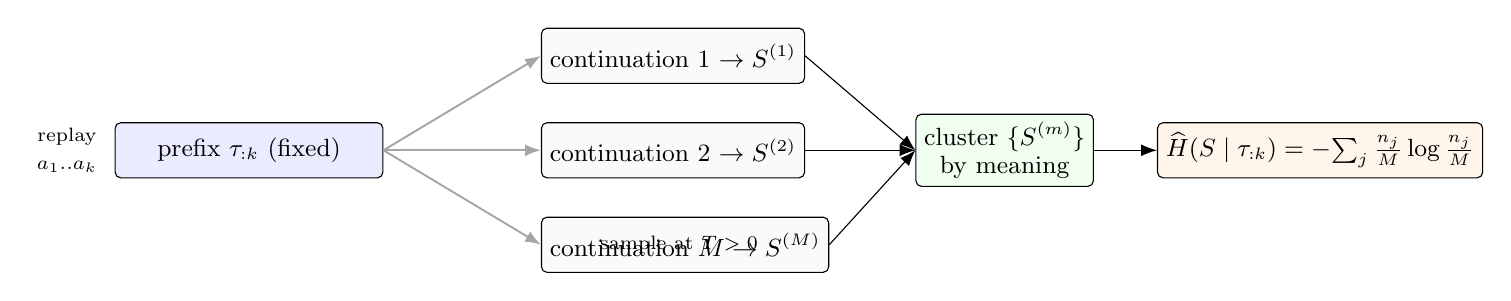
\begin{tikzpicture}[
  font=\small,
  box/.style={draw,rounded corners=2pt,inner sep=3pt,minimum height=7mm},
  cont/.style={-{Latex[length=2mm]},gray!70,line width=0.7pt},
  >={Latex[length=2mm]}]
% prefix bar
\node[box,fill=blue!8,minimum width=34mm] (pre) {prefix $\tau_{:k}$ (fixed)};
\node[left=1mm of pre,align=center] {\scriptsize replay\\[-1pt]\scriptsize $a_1..a_k$};
% fork point
\coordinate (fork) at ($(pre.east)+(4mm,0)$);
\node[right=20mm of pre,yshift=12mm,box,fill=gray!4] (c1) {continuation 1 $\to S^{(1)}$};
\node[right=20mm of pre,yshift=0mm,box,fill=gray!4]  (c2) {continuation 2 $\to S^{(2)}$};
\node[right=20mm of pre,yshift=-12mm,box,fill=gray!4](cm) {continuation $M \to S^{(M)}$};
\draw[cont] (pre.east) -- (c1.west);
\draw[cont] (pre.east) -- (c2.west);
\draw[cont] (pre.east) -- (cm.west);
\node at ($(c2)!0.5!(cm)+(0,-6mm)$) {\scriptsize sample at $T>0$};
% cluster + entropy
\node[right=14mm of c2,box,fill=green!6,align=center] (cl)
   {cluster $\{S^{(m)}\}$\\[-1pt]by meaning};
\draw[->] (c1.east) -- (cl.west);
\draw[->] (c2.east) -- (cl.west);
\draw[->] (cm.east) -- (cl.west);
\node[right=8mm of cl,box,fill=orange!8] (H)
   {$\Hk=-\!\sum_j \tfrac{n_j}{M}\log\tfrac{n_j}{M}$};
\draw[->] (cl.east) -- (H.west);
\end{tikzpicture}
\caption{\textbf{Interventional estimator of $H(S\mid\tau_{:k})$.} The first $k$
steps are fixed (reconstructed by deterministic replay), then $M$ continuations
are sampled to completion. Their final strategies $S^{(m)}$ are clustered by
meaning and the discrete semantic entropy is computed. Sweeping $k$ traces the
commitment curve.}
\label{fig:method}
\end{figure}

\section{Related work}
\label{sec:related}

\paragraph{Commitment as a collapsing curve is an old idea.}
Across fields, the uncertainty of a sequential process's outcome falls as the
process unfolds, after which the result is effectively determined. Chemical physics
makes this precise with the \emph{committor} of transition-path theory: $q(x)$, the
probability a trajectory from microstate $x$ reaches the product basin before the
reactant, runs from $0$ to $1$ along a reactive path; its $q\!=\!\tfrac12$
iso-surface is the \emph{transition state}; and it is regarded as the ideal
one-dimensional reaction coordinate~\citep{evanden2010tpt}. The information
thermodynamics of the transition-path ensemble further ties entropy production to
how much the dynamics reveal about a trajectory's
reactivity~\citep{louwerse2022infothermo}. The same collapsing shape appears as
sports win-probability curves that flatten as a game progresses~\citep{brill2024winprob}
and as the empirical predictability of LLM reinforcement-learning trajectories from
early states~\citep{cai2025predictability}. We adopt this lineage explicitly:
$\Hk$ is an entropy-generalized committor for agent trajectories. What it adds is a
feature absent when---as in physics---the sampler and the dynamics are the same
object: a \emph{learned} generator can stop exploring before the outcome is
dynamically fixed, splitting the single collapse into the pair
$(f^\ast,f^\dagger)$.

\paragraph{Irreversibility and option value in RL.}
The $f^\dagger$ side---an outcome becoming unreachable---is the subject of
reversibility-aware RL, which learns which action sequences cannot be
undone~\citep{grinsztajn2021noreturn}, and of the \emph{power}/\emph{empowerment}
literature, where keeping many futures reachable is instrumentally
valuable~\citep{turner2019power} and is now estimated for language-model agents
directly~\citep{song2025empowerment}. These quantify the reachability of \emph{states};
we instead track the entropy of the final \emph{executed outcome}, and we pair its
causal-lock threshold with the generator's collapse threshold---a separation the
reachability view does not make.

\paragraph{Diversity and forking in language models.}
Closest to our mechanism, Bigelow et al.~\citep{bigelow2024forking} resample
single-turn generations token-by-token and use Bayesian change-point detection to locate
\emph{forking tokens} where the final-answer distribution shifts, summarized by a
\emph{survival function} $S(T)$. We differ on four axes that matter for the agent
setting: their analysis is single-turn and token-level, ours is over a multi-step
agent's trajectory prefixes; their outcomes are one-hot answers, LLM-extracted text,
or embeddings, whereas ours are \emph{executed} behavioral signatures (the
test-outcome vector a patch induces), giving a non-circular, non-learned meaning
relation; they measure one curve under forced resampling, we separate the
generator-collapse ($f^\ast$) and outcome-lock ($f^\dagger$) thresholds; and we turn
the result into a test-time-compute policy (inject in $[f^\ast,f^\dagger)$). A
parallel training-time line finds that a sparse set of high-entropy
``forking''/``critical'' tokens decides reasoning
direction~\citep{wang2025highentropy,lin2024critical} and trains models to branch at
them~\citep{jia2025globalforking}; these corroborate our premise---decision-bearing
positions are sparse and the diverse-but-correct forks sit deep in the
trajectory, predicting a non-trivial $f^\ast$---but they operate on the training
loss, remain single-turn, and never measure \emph{where} branching pays. Finally,
the inference-time uncertainty gates for agents discussed
above~\citep{egb2025,catts2026,learnwhentoplan2025} are complementary: they
approximate, online and locally, the interventional quantity we measure offline.

\section{Methods}

\subsection{Setup and what we mean by ``strategy''}
We study a ReAct-style agent~\citep{yao2023react} that solves a task by emitting a
sequence of steps $\tau=(a_1,o_1,\dots,a_T,o_T)$, where each $a_t$ contains
reasoning and a single shell action and $o_t$ is the resulting observation; the
episode terminates when the agent submits a patch. Our primary model is
Qwen3-Coder-30B served locally; for the cross-model landscape analysis
(\S\ref{sec:landscape}) we add a panel of open code models. Tasks are drawn from
SWE-bench Verified~\citep{jimenez2024swebench} (SymPy), with one isolated container
per trajectory.

The outcome of a trajectory is its \textbf{final patch}, and the entropy in
\S\ref{sec:measure} is taken over \emph{meaning classes} of patches. The crucial
point is that, because our outputs are executable programs, ``same meaning'' is
not a free-text judgment but a \emph{checkable} one: two patches mean the same
thing if they make the repository \emph{behave} the same way. We define the
meaning map as a hierarchy from coarse to fine (\S\ref{sec:instrument}): (i)
\textbf{resolution}---resolved vs.\ not (one bit); (ii) \textbf{behavioral
signature}---the vector of per-test outcomes a patch induces, optionally augmented
by hashed differential-test outputs; and (iii) \textbf{structural}---which
files, functions, and hunks the patch changes. All three are deterministic and
require no learned text-similarity. Behavioral equivalence (ii) is the
principled backbone: two textually different patches that flip the same tests are
the same outcome (renamings, reordered independent edits, caller- vs.\ callee-side
fixes), and two near-identical patches that differ on a test are different
outcomes---distinctions that surface-level diffing gets backwards. This relation
is unavailable to text-only semantic-entropy work; here we can run the code.
Structural equivalence (iii) is a finer, deterministic refinement used as a
secondary lens---it separates two genuinely different \emph{approaches} that
happen to behave identically. In all cases the patch---not the long,
scaffold-dominated, order-sensitive trajectory---is the unit of meaning.

\subsection{Conditional outcome entropy and commitment}
\label{sec:measure}
Let the agent define a stochastic policy $\pi$ at sampling temperature $T$, so the
final strategy $\strat$ (the patch) is a random variable. Fix a prefix
$\prefix=(a_1,o_1,\dots,a_k,o_k)$ of length $k$. We define the conditional
semantic entropy of the outcome given the prefix,
\begin{equation}
H(\strat \mid \prefix)\;=\;-\!\!\sum_{c \in \mathcal{C}} p(c\mid\prefix)\,\log p(c\mid\prefix),
\qquad
p(c\mid\prefix)=\Pr_{\,\text{cont}\sim\pi(\cdot\mid\prefix)}\!\big[\,\text{meaning}(\strat)=c\,\big],
\end{equation}
where $\mathcal{C}$ is the set of \emph{meaning classes} of final patches and the
meaning map is the behavioral (primary) / structural hierarchy of
\S\ref{sec:instrument}; we evaluate $\Hk$ at each granularity. Following discrete
semantic entropy~\citep{farquhar2024semantic,kuhn2023semantic}, the quantity is
defined over meaning classes rather than surface forms and requires no token
probabilities. Read along the reference trajectory, $\Hk$ is the \emph{cumulative}
diversity still reachable from step $k$ by plain resampling---a statement about the
outcome, not yet about any individual step's role in deciding it.

\paragraph{What licenses an injection: per-step leverage.}
The cumulative curve is not yet the object we want, because injecting diversity at
step $k$ changes the outcome only insofar as step $k$ actually \emph{decides} it.
The quantity that measures this---our \emph{primary} object---is the conditional
mutual information between the step's action $A_k$ and the final outcome, given the
prefix, $\ell_k = I(A_k;\strat\mid\tau_{:k-1})$. By the elementary bound that mutual
information cannot exceed either marginal entropy~\citep{cover2006elements},
\begin{equation}
\ell_k \;\le\; \min\big(\,H(A_k\mid\tau_{:k-1}),\;\; H(\strat\mid\tau_{:k-1})\,\big).
\end{equation}
Leverage is appreciable only where the step is itself \emph{branchy}
($H(A_k\mid\tau_{:k-1})$ large---the model has genuinely different actions available)
\emph{and} the outcome is still \emph{open} ($H(\strat\mid\tau_{:k-1})$ large---there
is something left to decide). This is the formal content of the balance between
conditioning and uncertainty: leverage vanishes at both ends of a trajectory for
\emph{opposite} reasons---at deterministic ``boilerplate'' steps (read the obvious
file, run the suite) the first term is $\approx\!0$, so the step decides nothing
however open the outcome; once the outcome is fixed the second term is $0$, so even a
branchy step is inconsequential. In particular, injecting at the very first step is
typically wasteful not because diversity is cheap there but because the opening
action is forced by the repository ($H(A_1\mid\tau_{:0})\!\approx\!0$) even though the
outcome is maximally open. The profile $\{\ell_k\}$ is therefore generally uneven and
multi-peaked, a few scattered steps carrying most of the commitment; we do
\emph{not} assume a single wide-to-narrow sweep. Averaged over a step's
realizations $\ell_k$ equals the expected drop in outcome entropy (chain rule of
mutual information~\citep{cover2006elements}), but along a \emph{single} reference the
realized increment $H(\strat\mid\tau_{:k-1})-H(\strat\mid\tau_{:k})$ can be
\emph{negative}---a step that inspects code may reveal that several repairs are
viable---so it is only an expectation-level proxy for $\ell_k$.

\paragraph{Two summary thresholds, stated honestly in support.}
Two scalars bracket where injection can help. They are cleanest in terms of the
\emph{support} of the outcome distribution (the classes with positive probability),
for which a rigorous ordering holds; entropy alone does not give one. Let
$\mathrm{supp}_\pi(k)$ be the outcome classes reachable by plain resampling from
$\tau_{:k}$, and $\mathrm{R}(k)$ those reachable by \emph{any} admissible
intervention on the next step followed by resampling. Plain resampling is one such
intervention, so $\mathrm{supp}_\pi(k)\subseteq \mathrm{R}(k)$ at every $k$. Define
\begin{equation}
f^\ast=\sup\{\,k/T : |\mathrm{supp}_\pi(k)|>1\,\},\qquad
f^\dagger=\sup\{\,k/T : |\mathrm{R}(k)|>1\,\},
\end{equation}
the \emph{last} prefix fraction at which plain resampling, respectively any
intervention, still yields more than one outcome (the last upcrossing, not the first
dip, since the curves are non-monotone). The inclusion
$\mathrm{supp}_\pi\subseteq\mathrm{R}$ gives $f^\ast\le f^\dagger$
\emph{rigorously}: if no intervention can move the outcome, plain resampling
certainly cannot. We deliberately avoid the stronger-looking claim that the forced
entropy dominates the natural one pointwise---forcing one particular action can
\emph{lower} outcome entropy---so the inequality we rely on is the support
inclusion, with entropy used only as a graded read-out. The \emph{injectable set}
$\{k:\,|\mathrm{supp}_\pi(k)|=1<|\mathrm{R}(k)|\}$---resampling collapsed but an
intervention still reaches alternatives---lies in $[f^\ast,f^\dagger)$ but need
\emph{not} be a contiguous interval. The claim $f^\ast<f^\dagger$ is exactly that
the model commits (its resampling support collapses) before the problem locks (its
reachable support collapses); $f^\dagger$ is reported relative to the forcing
operator actually used---a lower bound on true reachability (\S\ref{sec:protocol}).

\paragraph{A reaction coordinate: aligning by resolved entropy.}
Indexing by prefix fraction $k/T$ is lossy: the same decision can occur at step $3$
of one trajectory and step $7$ of another, so averaging by $k/T$ smears distinct
decisions together. Transition-path theory meets the same problem and indexes not by
time but by the committor, the reaction coordinate measuring progress through the
transition~\citep{evanden2010tpt}. Its analogue here is the \emph{fraction of outcome
entropy resolved},
\begin{equation}
\rho(k)\;=\;1-\frac{H(\strat\mid\tau_{:k})}{H(\strat\mid\tau_{:0})}\;\in[0,1]
\qquad (H(\strat\mid\tau_{:0})>0),
\end{equation}
$0$ when nothing is decided, $1$ at lock-in. We report the leverage profile and the
thresholds against $\rho$ as well as $k/T$, so commitment events align across
trajectories by \emph{how far the outcome has been decided} rather than by wall-clock
step. ($\rho$ is monotone only in expectation and estimated with noise; we use it as
a coordinate, never as a quantity to optimize.)

\paragraph{Estimator.}
From a prefix $\prefix$ we draw $M$ continuations
$\text{cont}^{(1)},\dots,\text{cont}^{(M)}\sim\pi(\cdot\mid\prefix)$, cluster their
final patches into classes $\{C_j\}$ of sizes $n_j$, and form the plug-in discrete
entropy
\begin{equation}
\Hk \;=\; -\sum_j \frac{n_j}{M}\,\log\frac{n_j}{M}, \qquad
\Hk^{\text{norm}} \;=\; \Hk\,/\,\log M .
\label{eq:estimator}
\end{equation}
Evaluating this at successive prefixes along the reference traces the natural curve
$H(\strat\mid\tau_{:k})$ and its support $\mathrm{supp}_\pi(k)$; repeating with a
forced maximally-diverse first action traces the reachable surrogate
$\mathrm{R}(k)$. The per-step leverage $\ell_k$ is read two ways: cheaply, as the
curve increment $\Delta_k=\widehat H(\strat\mid\tau_{:k-1})-\widehat
H(\strat\mid\tau_{:k})$, an expectation-level proxy that can go negative; and, on a
cost-limited subset of steps, by a \emph{direct nested} estimate of the mutual
information itself---draw $R$ alternative actions
$a_k^{(1)},\dots,a_k^{(R)}\sim\pi(\cdot\mid\tau_{:k-1})$, continue each $M$ times to
outcome distributions $\hat p_r$, and form the Jensen--Shannon-type information
$\widehat\ell_k = H\!\big(\tfrac1R\textstyle\sum_r \hat p_r\big)-\tfrac1R\sum_r
H(\hat p_r)$. Plug-in entropies are biased low at small $M$; we apply the
Miller--Madow correction and report $\log M$ as the ceiling. The estimator is
\textbf{non-circular} (it references only counterfactual continuations, never the
realized final) and \textbf{interventional} (fixing $\prefix$ and resampling is a
$\mathrm{do}(\cdot)$ on the prefix). It is monotone \textbf{only in expectation}:
$\mathbb{E}[H(\strat\mid\tau_{:k})]$ is non-increasing in $k$ because conditioning
cannot raise average entropy~\citep{cover2006elements}, but the single-reference
curve we measure can rise locally---which is why the thresholds are defined by
sustained collapse and the leverage profile, not a first crossing, is the object of
record.

\paragraph{A second axis: path entropy.}
The curve $\Hk$ measures the diversity of \emph{where} a trajectory ends.
Orthogonal to it is the diversity of \emph{how} it reaches a given end---the
path-conditional entropy $H(\text{path}\mid \strat{=}c)$, which we summarize by the
dispersion (pairwise structural similarity and length) of the continuations that
land in a fixed class $c$. A class reached by many dissimilar paths is robustly
``canalized-to''; one reached by a single path is brittle. Outcome entropy and
path entropy are independent---a problem may admit one outcome reached a hundred
ways, or ten outcomes each reached one way---and a single scalar conflates them, so
we report both (\S\ref{sec:landscape}).

\subsection{Reconstructing the prefix by deterministic replay}
\label{sec:replay}
Sampling $\pi(\cdot\mid\prefix)$ requires placing the agent in the exact state
after $k$ steps---crucially, the container filesystem written by $a_1,\dots,a_k$,
not merely the textual history. We reconstruct this state by \emph{deterministic
replay}: we instantiate a fresh evaluation container and re-execute the recorded
shell actions $a_1,\dots,a_k$ (deterministic file-reading/writing commands),
which reproduces the on-disk state, and we set the agent's message history to
$\prefix$. Replay avoids storing a container image per step and yields the exact
prefix state; continuations then proceed by ordinary sampling at temperature $T$.
A single reference trajectory per problem (greedy decoding, $T=0$) defines the
prefixes to be reconstructed.

\subsection{Meaning equivalence: behavioral and structural signatures}
\label{sec:instrument}
The entropy in Eq.~\eqref{eq:estimator} is taken over \emph{meaning classes}, so
it depends entirely on the relation that decides when two final patches mean the
same thing. Because our outputs are executable, we take this relation to be
\textbf{behavioral} as the principled primary: we run the patched repository
against the instance's tests and assign each patch its \emph{behavioral
signature}---the vector of per-test outcomes over the \textsc{fail\_to\_pass} and
\textsc{pass\_to\_pass} tests, optionally augmented by hashed outputs of
additional differential inputs. Two patches share a class iff they share a
signature. This collapses behaviorally-equivalent patches that surface diffing
over-counts (renamings, reordered independent edits, caller- vs.\ callee-side
fixes) and separates near-identical patches that flip a test, and it is obtained
essentially for free: the evaluation harness already executes these tests. One
caveat is inherent: behavioral equivalence is defined \emph{relative to the test
suite}---two patches agreeing on every test may differ on untested inputs. For
SWE-bench the curated suite is the task's behavioral specification, so the
relation is principled though coarse; differential or property testing sharpens it
where needed.

A finer, \emph{structural} refinement separates two genuinely different
\emph{approaches} that nonetheless behave identically---for instance a fix in the
caller versus the callee that passes exactly the same tests. We obtain it
deterministically from the patch itself: the set of files, functions, and hunks it
touches (its structural signature), with two patches refined into the same class
when they edit the same code locations in the same way. Crucially, this needs no
\emph{learned text-similarity}. The whole meaning hierarchy is therefore free of
model judgment: the primary relation is \emph{executed} (a test-outcome signature)
and the refinement is \emph{parsed} (a structural signature), so neither the
generative model nor any auxiliary similarity model adjudicates what counts as
``the same.'' This is a deliberate departure from the text-similarity clustering of
semantic-entropy work on free-form answers~\citep{farquhar2024semantic,kuhn2023semantic},
which is neither available nor necessary once the outputs are programs we can run
and parse.

\subsection{Beyond a single model: the outcome landscape}
\label{sec:landscape}
A single model's commitment curve is confounded. A uniformly low $\Hk$ is
consistent with two opposite situations: the problem genuinely admits one solution
and the model commits to it immediately, or the problem admits many but the model
is mode-collapsed onto one~\citep{zhang2025noveltybench}. From one model these are
indistinguishable---a flat low curve reads as early commitment but may be mere
narrowness. The remedy is a \emph{reference frame}. Let a panel of models
$\{m_1,\dots,m_P\}$ each produce outcomes for a problem; merging their outcomes
under the meaning relation of \S\ref{sec:instrument} yields the problem's
\emph{outcome landscape} $\Lambda$, an estimate of the set of behaviorally distinct
viable solutions. Against $\Lambda$ the single-model quantities become
interpretable: \emph{commitment} corresponds to a small $\Lambda$ (the problem
really has few solutions), \emph{collapse} to a large $\Lambda$ of which the model
covers only a corner. We summarize this with each model's \emph{coverage}
$\lvert\mathcal{C}_m\rvert/\lvert\Lambda\rvert$ and the cross-model class-overlap
matrix, which separates \emph{convergent} models (reaching the same classes) from
\emph{complementary} ones (reaching disjoint classes---the regime where ensembling
helps).

\paragraph{Statistics logged.}
For each (model, problem) we record the per-step \emph{leverage} profile
$\{\ell_k\}$ (the curve increment $\Delta_k$ at every step, plus the direct nested
estimate on a step subset), the natural and reachable outcome-support curves with
the summary pair $(f^\ast,f^\dagger)$ and the injectable \emph{set} between them, and
the resolved-entropy coordinate $\rho(k)$; together with the \emph{cost of
commitment} (turns and tokens until the natural support first collapses to one
class), the number of outcome classes, and, per class, its probability and
intra-class path similarity (the path axis of \S\ref{sec:measure}). For each problem
we record the landscape size $\lvert\Lambda\rvert$, per-model coverage, and the
cross-model overlap matrix. All are computed from artifacts the runs already
produce.

\subsection{Pre-registered protocol}
\label{sec:protocol}
We fix the following before running, to avoid post-hoc tuning:
\begin{itemize}[leftmargin=1.4em,itemsep=2pt,topsep=2pt]
\item \textbf{Reference \& prefixes.} One greedy reference trajectory per problem.
For the leverage profile we resample at \emph{every} step where the trajectory is
short and on a fixed stride otherwise (the stride is fixed in advance and reported),
with $k\!=\!0$ the maximal-openness anchor; the cheap increment $\Delta_k$ is
computed at all swept prefixes and the direct nested estimate $\widehat\ell_k$ on a
pre-declared step subset.
\item \textbf{Continuations.} $M$ continuations per prefix at $T=0.7$ (the
model's recommended sampling temperature), drawn twice per prefix---once plain (for
$H(\strat\mid\tau_{:k})$ and the natural support $\mathrm{supp}_\pi$, giving
$f^\ast$) and once with a forced maximally-different next action (for the reachable
support $\mathrm{R}$, giving $f^\dagger$); the nested estimate additionally draws $R$
actions per subset step. One container alive at a time.
\item \textbf{Outcome \& meaning.} Final patch; \emph{primary} meaning relation =
behavioral signature (per-test outcome vector); \emph{secondary} = structural
signature (files/functions/hunks changed); entropy by Eq.~\eqref{eq:estimator} at
each granularity, with Miller--Madow correction.
\item \textbf{Models.} A primary model (Qwen3-Coder-30B) for the commitment curves;
a panel of open code models for the outcome-landscape analysis
(\S\ref{sec:landscape}), served one at a time. As a pre-registered
\emph{family-generality} test we require this panel to span $\geq\!2$ coder
\emph{families} (at least one non-Qwen, e.g.\ a DeepSeek- or Llama-class 30B coder):
lock-in is model-dependent, present for some models and absent for
others~\citep{entropydynamics2026}, and aligned-model diversity collapse varies by
lineage~\citep{diversitycollapse2025,zhang2025noveltybench}, so $f^\ast$ is a
\emph{per-family} quantity that must be sampled across families rather than assumed
constant. We report $(f^\ast,f^\dagger)$ per family on the resolved-entropy axis with
the forcing operator stated per family ($f^\dagger$ is operator-relative); the support
inclusion $\mathrm{supp}_\pi(k)\subseteq\mathrm{R}(k)$ holds within every family
regardless of lineage, so $f^\ast\le f^\dagger$ is guaranteed per family and any
inversion would signal an estimator bug, not a real effect. The open prediction is
that Qwen collapses earlier (smaller $f^\ast$) than a less-aligned family while the
window $[f^\ast,f^\dagger)$ stays non-empty for at least one non-Qwen family; the
injectable-window policy is Qwen-specific only if every non-Qwen family yields
$f^\ast\approx f^\dagger$. Like the cross-repo axis, this one is \emph{unfilled}: the
sole completed run is the single degenerate Qwen SymPy instance above ($n=1$,
$f^\ast=0$, $\widehat{H}_{\mathrm{MM}}=0$ at every measured fraction
$\{0,0.5,0.9\}$). Here $f^\ast=0$ is the \emph{unconditioned} collapse
$|\mathrm{supp}_\pi(0)|=1$: free resampling ($k=0$, no prefix fixed) already yielded
a single behavioral outcome class, so on this instance the natural-support arm is
uninformative and cannot localize a window. The cross-family panel therefore stands
at zero non-Qwen families: this run fixes neither $f^\ast$ for any family nor the
cross-family contrast, and $f^\dagger$ still awaits the forced-diverse
reachable-support run.
\item \textbf{Problems.} The SWE-bench Verified SymPy set, scaling to a larger and
more diverse array; all claims scoped to the set actually run. As a pre-registered
\emph{scope-generality} test---generalizing single-repository entropy-at-decision-point
evidence~\citep{egb2025,catts2026} to a cross-repository commitment claim---we extend
the estimator to $8$--$10$ instances from each of $\geq\!2$ further SWE-bench
repositories beyond SymPy (e.g.\ \textsc{django}, \textsc{scikit-learn}/\textsc{matplotlib})
and report per-repo $(f^\ast,f^\dagger)$ and the rarefaction-corrected entropy curve.
The support inclusion $\mathrm{supp}_\pi(k)\subseteq\mathrm{R}(k)$ holds within each
repository independently of codebase, so $f^\ast\le f^\dagger$ is guaranteed
per repo by support inclusion---making the \emph{ordering} domain-invariant
\emph{a priori}, so that a second-repository arm can test only the window's
\emph{magnitude} (its location and width), never the sign---and any observed
inversion $f^\ast>f^\dagger$ would
signal an estimator bug rather than a real effect; the open prediction is that the
\emph{window width} $[f^\ast,f^\dagger)$ varies across codebases (wider where an issue
admits several fix loci) while the ordering never inverts, with the framing failing
to generalize only if some repo yields $f^\ast>f^\dagger$ or all repos collapse to
$f^\ast=f^\dagger=$~trajectory-end. To date this axis is \emph{unfilled}: the sole run
is the single-instance SymPy estimator check above (\texttt{sympy-22714},
behavioral-signature clustering; $n=1$, $f^\ast=0$,
$\widehat{H}_{\mathrm{MM}}=0$ at every measured fraction $\{0,0.5,0.9\}$), which neither
establishes nor refutes cross-repo generality---and, being degenerate, supplies no
nonzero SymPy baseline against which a second repository could be compared: with all
$\ell_k=0$ the predicted leverage-concentration check (Gini of $\{\ell_k\}>0.5$) is
undefined, and $f^\dagger$ awaits the forced-diverse reachable-support run.
The comparison must moreover respect a per-repository constraint: because behavioral
equivalence is defined relative to each instance's \emph{own} held-out suite
(\S\ref{sec:instrument}), signatures are computed per-suite and are never compared
across repositories; the ordering $f^\ast\le f^\dagger$ is read \emph{within} each
repo, and only the \emph{shape} of its curves---not the outcome classes
themselves---transfers across the panel. This also bounds what such a panel could
extend: prior survival/change-point evidence of collapse is single-turn and
single-domain~\citep{bigelow2024forking}, so a cross-repo result would extend that
collapse phenomenon to a multi-step agent over structurally distinct codebases.
The cross-repo comparison therefore remains entirely to be produced.
\item \textbf{Primary analysis.} The per-step leverage profile $\{\ell_k\}$ and the
natural/reachable support curves, plotted against both $k/T$ and the resolved-entropy
coordinate $\rho$; the joint distribution of $(f^\ast,f^\dagger)$ and the prevalence,
size, and \emph{contiguity} of the injectable set (is it a band or dispersed?);
per-problem heterogeneity (early- vs.\ late-committing, Figure~\ref{fig:concept});
and, across the panel, the outcome landscape $\lvert\Lambda\rvert$, per-model
coverage, the path-entropy axis, and commitment-cost statistics
(\S\ref{sec:landscape}).
\end{itemize}

\paragraph{Hierarchy and ordering (secondary analysis).}
Because a strategy is an overall approach plus an ordered composition of
substrategies, two trajectories can reach the same approach by different routes
(reordered substeps) or diverge in substrategy while sharing an approach. The
patch-level outcome answers the \emph{overall-approach} question directly. To probe
the substrategy layer we will additionally decompose each continuation into a
sequence of sub-intents and compare sequences with an order-aware transport
distance, reported separately; this layer is exploratory and does not affect the
primary curve.

\paragraph{Anticipated threats to validity.}
(i) \emph{Reference dependence}: $f^\ast$ conditions on one reference prefix per
problem; we will quantify sensitivity by repeating with sampled references on a
subset. (ii) \emph{Estimator bias and the leverage proxy}: small $M$ biases plug-in
entropy low (we report Miller--Madow-corrected values and $\log M$ as the ceiling);
moreover the cheap increment $\Delta_k$ estimates per-step leverage only in
expectation and can go negative along a single reference, so we treat it as a screen
and confirm flagged steps with the direct nested estimate $\widehat\ell_k$. (iii)
\emph{Support and coordinate sensitivity}: the support-based thresholds
$f^\ast,f^\dagger$ depend on $\varepsilon$ and $M$---a rare outcome class surfaces
only with more samples and can push a threshold later---and $\rho$ is computed from
noisy entropy estimates; we report threshold sensitivity to $(\varepsilon,M)$ and
present results in both $k/T$ and $\rho$. (iv)
\emph{Replay fidelity}: nondeterministic commands could perturb the reconstructed
state; we restrict replay to the recorded deterministic actions and verify state
equivalence on spot checks. (v) \emph{Landscape under-coverage}: the outcome
landscape $\Lambda$ is a \emph{lower bound} estimated from a finite model panel and
finite sampling, so coverage figures are relative to it; a larger panel can only
enlarge $\Lambda$. (vi) \emph{Intervention dependence}: $f^\dagger$ and the
injectable set are defined relative to a particular forced-diversity operator (a
strategy-proposal injection), so they are a \emph{lower bound} on true
reachability---a stronger intervention can only push $f^\dagger$ later and widen the
set; we report the operator explicitly and treat $f^\dagger$ as operator-relative,
not absolute. (vii) \emph{Scope}: results are scoped to the problem set and
model panel actually run; the measure itself is model-agnostic. (viii)
\emph{Instrument reproducibility}: every value of $\Hk$ inherits the reproducibility
of the meaning instrument that defines its classes---if a patch's behavioral
signature is not stable across repeated suite executions, cluster assignments and
hence the entropy are instrument noise rather than commitment. This assumption is
logically prior to the entropy and must be validated by \emph{rerun-reproducibility},
not by the curve it later produces. We therefore pre-register an instrument check
independent of any commitment claim: on the patches already produced, execute each
instance's suite $K\!=\!5$ times in isolated containers, report per-test flakiness,
mask non-deterministic tests (behavioral equivalence is defined relative to the
suite, \S\ref{sec:instrument}), and measure the adjusted Rand index (ARI) of
behavioral clusters across reruns; the same ARI for NLI clustering on raw patch text
is the contrast, predicted lower, corroborating execution- over text-based meaning
for code~\citep{farquhar2024semantic,kuhn2023semantic}. The sole completed run cannot
exercise this check: with a single behavioral class ($f^\ast=0$,
$\widehat{H}_{\mathrm{MM}}=0$ throughout) the cluster partition is trivial and its
across-rerun ARI is degenerate (undefined / vacuously $1$), so instrument
reproducibility remains \emph{unverified}. The falsifier---signatures unstable across
identical reruns (ARI $<0.9$ after flaky-test masking)---would mean the meaning
classes, and with them every $\Hk$, are ill-defined and would require redefining the
instrument before any curve is interpretable.

\begin{figure}[t]
\centering
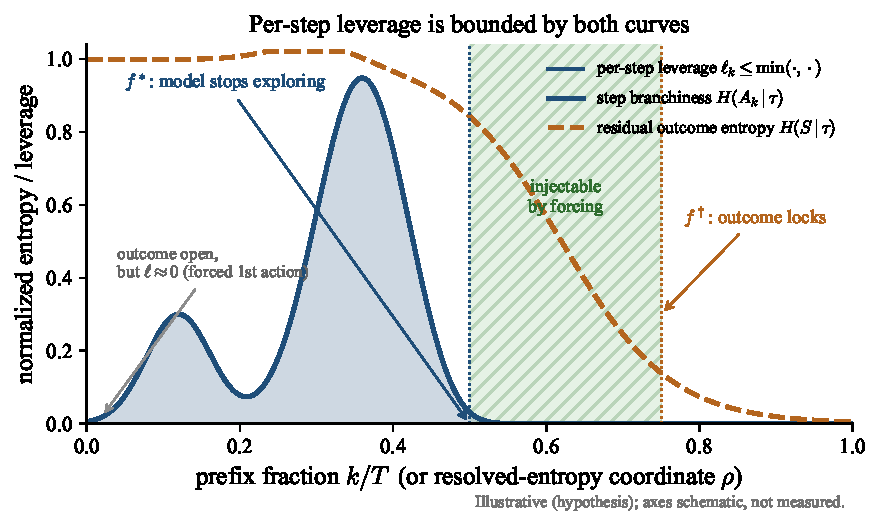
\includegraphics[width=0.74\linewidth]{commitment_concept.pdf}
\caption{\textbf{Hypothesis the experiment tests.} Per-step leverage
$\ell_k=I(A_k;\strat\mid\tau_{:k-1})$ (filled) is bounded by \emph{both} the step's
branchiness $H(A_k\mid\tau)$ (solid; is the model still exploring?) and the residual
outcome entropy $H(\strat\mid\tau)$ (dashed; is anything left to decide?), so it is
uneven and multi-peaked and vanishes at both ends for opposite reasons: the opening
action is near-deterministic (leverage $\approx0$ though the outcome is wide open),
and once the outcome is fixed even a branchy step is inconsequential. Branchiness
collapses at $f^\ast$ (the model stops exploring; natural support $\to 1$); residual
entropy collapses later at $f^\dagger$ (the outcome locks; reachable support $\to
1$). The hatched region $[f^\ast,f^\dagger)$ is injectable by \emph{forcing}---natural
exploration is spent but the outcome is still reachable---and need not be contiguous.
$f^\ast<f^\dagger$ is the model committing before the problem locks.
\emph{Schematic; not measured.}}
\label{fig:concept}
\end{figure}

\section*{Status}
This draft presents the idea, the measure, and the protocol for review prior to
any outcome experiments. The estimator, the prefix-replay harness, and the
behavioral/structural meaning relations are implemented; the commitment-curve and
outcome-landscape runs are withheld pending sign-off on the design.

\paragraph{Estimator check (single instance, natural support only; not an outcome
result).}
As an implementation check on the natural-support estimator---\emph{not} a test of
the commitment hypothesis---we ran it on a single instance
(\texttt{sympy\_\_sympy-22714}) with behavioral-signature clustering. The run
exercises the full behavioral pipeline end-to-end (prefix replay $\to$ continuation
resampling $\to$ test-outcome-signature clustering), confirming the estimator
executes on a real instance; it supplies no diversity signal. The estimate
is $f^\ast=0$: at every measured prefix fraction ($k/T\in\{0.0,0.5,0.9\}$) the
Miller--Madow-corrected conditional outcome entropy is
$\widehat{H}_{\mathrm{MM}}(\strat\mid\prefix)=0$, i.e.\ the resampled continuations
already collapse to a single behavioral outcome class at the earliest measured
prefix, so the natural support never exceeds one. We report this only to fix the
estimator's behavior and explicitly read it as a \emph{null}: with $n=1$ instance
and a single model it cannot separate an early-committing \emph{problem} from a
mode-collapsed \emph{model} (\S\ref{sec:landscape})---the precise confound the
cross-model panel exists to resolve, and one that is itself expected to be
model-dependent~\citep{entropydynamics2026,zhang2025noveltybench,diversitycollapse2025}.
The natural-support estimator moreover measures only where the model's \emph{own}
resampling spreads, not where the outcome is causally locked, so it bears on
$f^\ast$ alone. Because $n=1$, no across-instance bootstrap confidence interval on
$f^\ast$ is computable; we report one only once the instance count grows
(\S\ref{sec:protocol}). The lock prefix $f^\dagger$ is not yet estimable---it requires the
forced-diverse reachable-support run, which is not yet implemented---so the
injectable window $[f^\ast,f^\dagger)$ is left unreported, and no claim is made
about commitment from this point.

\begin{thebibliography}{99}
\small
\bibitem{yao2023react} S.~Yao et al. ReAct: Synergizing Reasoning and Acting in Language Models. \emph{ICLR}, 2023.
\bibitem{yang2024sweagent} J.~Yang et al. SWE-agent: Agent-Computer Interfaces Enable Automated Software Engineering. \emph{NeurIPS}, 2024.
\bibitem{jimenez2024swebench} C.~Jimenez et al. SWE-bench: Can Language Models Resolve Real-World GitHub Issues? \emph{ICLR}, 2024.
\bibitem{wang2023selfconsistency} X.~Wang et al. Self-Consistency Improves Chain of Thought Reasoning in Language Models. \emph{ICLR}, 2023.
\bibitem{yao2023tot} S.~Yao et al. Tree of Thoughts: Deliberate Problem Solving with Large Language Models. \emph{NeurIPS}, 2023.
\bibitem{zhou2023lats} A.~Zhou et al. Language Agent Tree Search Unifies Reasoning, Acting, and Planning. \emph{arXiv:2310.04406}, 2023.
\bibitem{snell2024scaling} C.~Snell et al. Scaling LLM Test-Time Compute Optimally\dots \emph{arXiv:2408.03314}, 2024.
\bibitem{zhang2025noveltybench} Y.~Zhang et al. NoveltyBench: Evaluating Language Models for Humanlike Diversity. \emph{COLM}, 2025.
\bibitem{farquhar2024semantic} S.~Farquhar et al. Detecting Hallucinations in Large Language Models Using Semantic Entropy. \emph{Nature}, 630:625--630, 2024.
\bibitem{kuhn2023semantic} L.~Kuhn et al. Semantic Uncertainty: Linguistic Invariances for Uncertainty Estimation. \emph{ICLR}, 2023.
\bibitem{egb2025} X.~Li, E.~Callanan, A.~Ghassel, X.~Zhu. Entropy-Gated Branching for Efficient Test-Time Reasoning. \emph{arXiv:2503.21961}, 2025.
\bibitem{learnwhentoplan2025} D.~Paglieri, B.~Cupia\l{}, J.~Cook, U.~Piterbarg, J.~Tuyls, E.~Grefenstette, J.~Foerster, J.~Parker-Holder, T.~Rockt\"aschel. Learning When to Plan: Efficiently Allocating Test-Time Compute for LLM Agents. \emph{arXiv:2509.03581}, 2025.
\bibitem{catts2026} N.~Lee, L.~E.~Erdogan, C.~J.~John, S.~Krishnapillai, M.~W.~Mahoney, K.~Keutzer, A.~Gholami. Agentic Test-Time Scaling for WebAgents. \emph{arXiv:2602.12276}, 2026.
\bibitem{diversitycollapse2025} L.~Yun, C.~An, Z.~Wang, L.~Peng, J.~Shang. The Price of Format: Diversity Collapse in Large Language Models. \emph{arXiv:2505.18949}, 2025.
\bibitem{entropydynamics2026} A.~Adeseye, A.~Adeseye, H.~Tenhunen, J.~Isoaho. Entropy and Attention Dynamics in Small Language Models: A Trace-Level Structural Analysis. \emph{Intelligent Systems Conf. (IntelliSys)}, 2026.
\bibitem{cover2006elements} T.~M.~Cover and J.~A.~Thomas. \emph{Elements of Information Theory}. Wiley, 2nd edition, 2006.
\bibitem{evanden2010tpt} W.~E and E.~Vanden-Eijnden. Transition-Path Theory and Path-Finding Algorithms. \emph{Annual Review of Physical Chemistry}, 61:391--420, 2010.
\bibitem{louwerse2022infothermo} M.~D.~Louwerse and D.~A.~Sivak. Information Thermodynamics of the Transition-Path Ensemble. \emph{Physical Review Letters} (arXiv:2106.11511), 2022.
\bibitem{brill2024winprob} R.~S.~Brill, R.~Yurko, A.~J.~Wyner. Exploring the Difficulty of Estimating Win Probability: A Simulation Study. \emph{arXiv:2406.16171}, 2024.
\bibitem{cai2025predictability} Y.~Cai, D.~Cao, X.~Xu, Z.~Yao, Y.~Huang, Z.~Tan, B.~Zhang, G.~Sun, G.~Liu, J.~Fang. On Predictability of Reinforcement Learning Dynamics for Large Language Models. \emph{arXiv:2510.00553}, 2025.
\bibitem{grinsztajn2021noreturn} N.~Grinsztajn, J.~Ferret, O.~Pietquin, P.~Preux, M.~Geist. There Is No Turning Back: A Self-Supervised Approach for Reversibility-Aware Reinforcement Learning. \emph{NeurIPS}, 2021.
\bibitem{turner2019power} A.~M.~Turner, L.~Smith, R.~Shah, A.~Critch, P.~Tadepalli. Optimal Policies Tend to Seek Power. \emph{NeurIPS} (arXiv:1912.01683), 2021.
\bibitem{song2025empowerment} J.~Song, J.~Gore, M.~Kleiman-Weiner. Estimating the Empowerment of Language Model Agents. \emph{arXiv:2509.22504}, 2025.
\bibitem{bigelow2024forking} E.~Bigelow, A.~Holtzman, H.~Tanaka, T.~Ullman. Forking Paths in Neural Text Generation. \emph{arXiv:2412.07961}, 2024.
\bibitem{wang2025highentropy} S.~Wang, L.~Yu, C.~Gao, C.~Zheng, S.~Liu, et al. Beyond the 80/20 Rule: High-Entropy Minority Tokens Drive Effective Reinforcement Learning for LLM Reasoning. \emph{arXiv:2506.01939}, 2025.
\bibitem{lin2024critical} Z.~Lin, T.~Liang, J.~Xu, Q.~Lin, X.~Wang, R.~Luo, C.~Shi, S.~Li, Y.~Yang, Z.~Tu. Critical Tokens Matter: Token-Level Contrastive Estimation Enhances LLM's Reasoning Capability. \emph{arXiv:2411.19943}, 2024.
\bibitem{jia2025globalforking} S.~Jia, X.~Wang, S.~P.~Kasiviswanathan. Training Large Language Models To Reason In Parallel With Global Forking Tokens. \emph{arXiv:2510.05132}, 2025.
\end{thebibliography}

\end{document}
